\documentclass[conference]{IEEEtran}

\usepackage[spanish]{babel}
\usepackage[utf8]{inputenc}
\usepackage{cite}
\usepackage{amsmath, amsthm,amssymb,amsfonts}
\usepackage{algorithmic}
\usepackage{graphicx}
\usepackage{textcomp}
\usepackage{xcolor}
\def\BibTeX{{\rm B\kern-.05em{\sc i\kern-.025em b}\kern-.08em
    T\kern-.1667em\lower.7ex\hbox{E}\kern-.125emX}}

% Definición del entorno 'definition'
\newtheorem{definition}{Definición}

\begin{document}
\title{Sistema Coordinado de Robots Industriales para Manipulación de Objetos\\
	% {\footnotesize \textsuperscript{*}Note: Sub-titles are not captured in Xplore and
	% should not be used}
	% \thanks{Identify applicable funding agency here. If none, delete this.}
}

\author{
	\IEEEauthorblockN{José Alejandro León Sánchez}
	\IEEEauthorblockA{\textit{Posgrado de Ingeniería} \\
		\textit{UNAM}\\
		CDMX, Mexico}
	\and
	\IEEEauthorblockN{Alejandro Rodríguez Angeles}
	\IEEEauthorblockA{\textit{CINVESTAV} \\
		\textit{IPN}\\
		CDMX, Mexico}
}

\maketitle

\begin{abstract}
	En esta ponencia se presentan avances en la teoría de control de robots para tareas de sincronización y coordinación de múltiples sistemas robóticos. A partir de los modelos dinámicos de robots industriales, se desarrollan esquemas de control en tiempo finito que aseguran la estabilidad y el cumplimiento de trayectorias bajo diversas condiciones operativas y restricciones de movimiento.
\end{abstract}

\begin{IEEEkeywords}
	Control de robots, sincronización, entorno, control de fuerza.
\end{IEEEkeywords}

\section*{Introducción}
El control de sincronización permite que múltiples robots trabajen de manera armónica, lo cual es crucial en aplicaciones industriales como ensamblaje o manipulación colaborativa. Sincronizar el movimiento implica un control preciso sobre la posición y velocidad de cada robot en relación con los demás. Los algoritmos de control más empleados incluyen métodos adaptativos y control por modos deslizantes, los cuales proporcionan robustez frente a variaciones en las propiedades físicas del sistema y el entorno.

\section*{Modelo Dinámico y Ecuaciones de Movimiento}
Los robots manipuladores se modelan a partir de sus ecuaciones dinámicas, las cuales describen su comportamiento bajo diferentes condiciones de carga y movimiento:

\begin{equation}
	M(q) \ddot{q} + C(q, \dot{q}) \dot{q} + \nabla_{q} U(q) = \tau,
\end{equation}

donde $M(q)$ representa la matriz de inercia, $C(q, \dot{q})$ el efecto de Coriolis, y $U(q)$ la energía potencial, actuando todos estos términos en el espacio articular de los robots.

Cuando los robots interactúan con su entorno, como al manipular objetos o moverse sobre superficies (Figura 1), se modela una fuerza de interacción \( h_r \), determinada por:

\begin{equation}
	h_{r} = M(\ddot{X} - \ddot{X}_{S}) + B(\dot{X} - \dot{X}_{S}) + K(X - X_{S}),
\end{equation}

donde $X_{S}$ es la posición de la superficie de contacto. Así, en presencia de restricciones de movimiento, el modelo se ajusta a:

\begin{equation}
	M(q) \ddot{q} + C(q, \dot{q}) \dot{q} + \nabla_{q} U(q) = \tau + J^{T}(q) h_{r}.
\end{equation}

\begin{figure}[h]
	\centering
	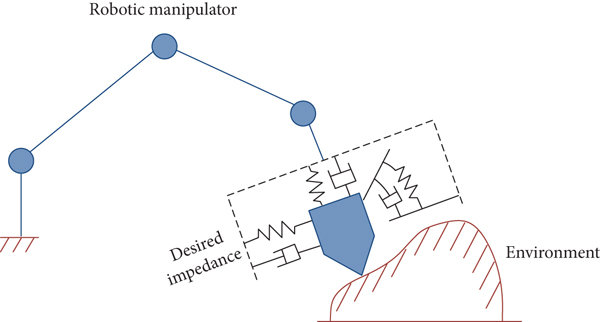
\includegraphics[width=0.5\textwidth]{robot-constrained.jpg}
	\caption{Representación de un robot con restricciones de movimiento en su entorno.}
\end{figure}

\section*{Estrategias de Control}
Para lograr la sincronización deseada y mantener el control de posición en el tiempo finito, se propone un controlador basado en PID, con términos adicionales de ajuste en los puntos de contacto para sistemas interactuando con el entorno. La ley de control toma la forma:

\begin{equation}
	\tau = K_{p} e_{q} + K_{i} \int e_{q} dt + K_{d} \dot{e_{q}},
\end{equation}

con ganancias \( K_{p}, K_{i}, K_{d} \) que se ajustan según las condiciones de operación. Para el control de fuerza, se aplican compensaciones adicionales que permiten un seguimiento robusto en sistemas con acoplamiento.

\begin{align}
	x_{P} & = K_{p p} e_{p} + K_{i p} \int e_{p} dt + K_{d p} \dot{e_{p}}, \\
	x_{f} & = K_{p f} e_{f} + K_{i f} \int e_{f} dt + K_{d f} \dot{e_{f}}.
\end{align}

\section*{Análisis de Estabilidad y Resultados}
Para la estabilidad de los sistemas acoplados, se utiliza el criterio de Routh-Hurwitz, evaluando las raíces del polinomio característico del sistema en lazo cerrado. Esta técnica asegura que el sistema se mantendrá estable incluso con variaciones en las condiciones de contacto y en la carga manipulada. En aplicaciones prácticas, el acoplamiento dinámico mejora el rendimiento al reducir los tiempos de ajuste y la respuesta ante perturbaciones externas.


\section*{Conclusiones}
El control de fuerza para robots manipuladores mejora significativamente la sincronización y coordinación en entornos colaborativos. Las futuras investigaciones se centrarán en implementar modelos de contacto más avanzados y desarrollar observadores de fuerza adaptativos para mejorar el rendimiento en tareas de manipulación con características complejas.

\begin{thebibliography}{9}
	\bibitem{aviles2017} Aviles, C. O. C., Díaz, A. M., \& Angeles, A. R., \textit{Control de Sincronización de un Robot Móvil Diferencial.}
	\bibitem{angeles2002} Angeles, A. R., \textit{Synchronization of mechanical systems} 2002.
	\bibitem{spong} M. W. Spong, S. Hutchinson, y M. Vidyasagar, *Robot Modeling and Control*. New York: John Wiley \& Sons, 2006.
\end{thebibliography}

\end{document}